I robot manipolatori collaborativi hanno rivoluzionato l'automazione industriale, permettendo lo svolgimento
di operazioni complesse in modo rapido, preciso e sicuro. 
La loro importanza nel campo dell'automazione industriale e di altre applicazioni \'{e} in continua crescita, con 
sempre pi\'{u} settori che ne riconoscono il valore e ne adottano l'utilizzo.
%Uno dei modelli pi\'{u} utilizzato \'{e} l'\textbf{UR5} di \textbf{Universal Robot}. Si \'{e} scelto di utilizzarlo in questo studio, 
%per via della sua flessibilit\'{a} ed efficienza. 
Un ruolo chiave nel controllo di questi robot viene assunto dai sensori coppia-forza,
che permettono di misurare e regolare la forza esercitata dal robot durante lo svolgimento delle proprie attivit\'{a}. 
La loro versatilit\'{a} li rende strumenti preziosi in molti campi della \textbf{robotica industriale} e della \textbf{medicina}. 
Essi infatti consentono al robot di controllare la forza esercitata durante operazioni di assemblaggio, levigatura, 
saldatura o manipolazione degli oggetti, come mostrato in Figura \ref{fig:industrial_applications}. 
Vengono inoltre utilizzati nella riabilitazione fisioterapica, per valutare la forza muscolare 
e i progressi del paziente. 
\begin{figure}[H]
    \centering
    \begin{subfigure}[b]{0.33\textwidth}
        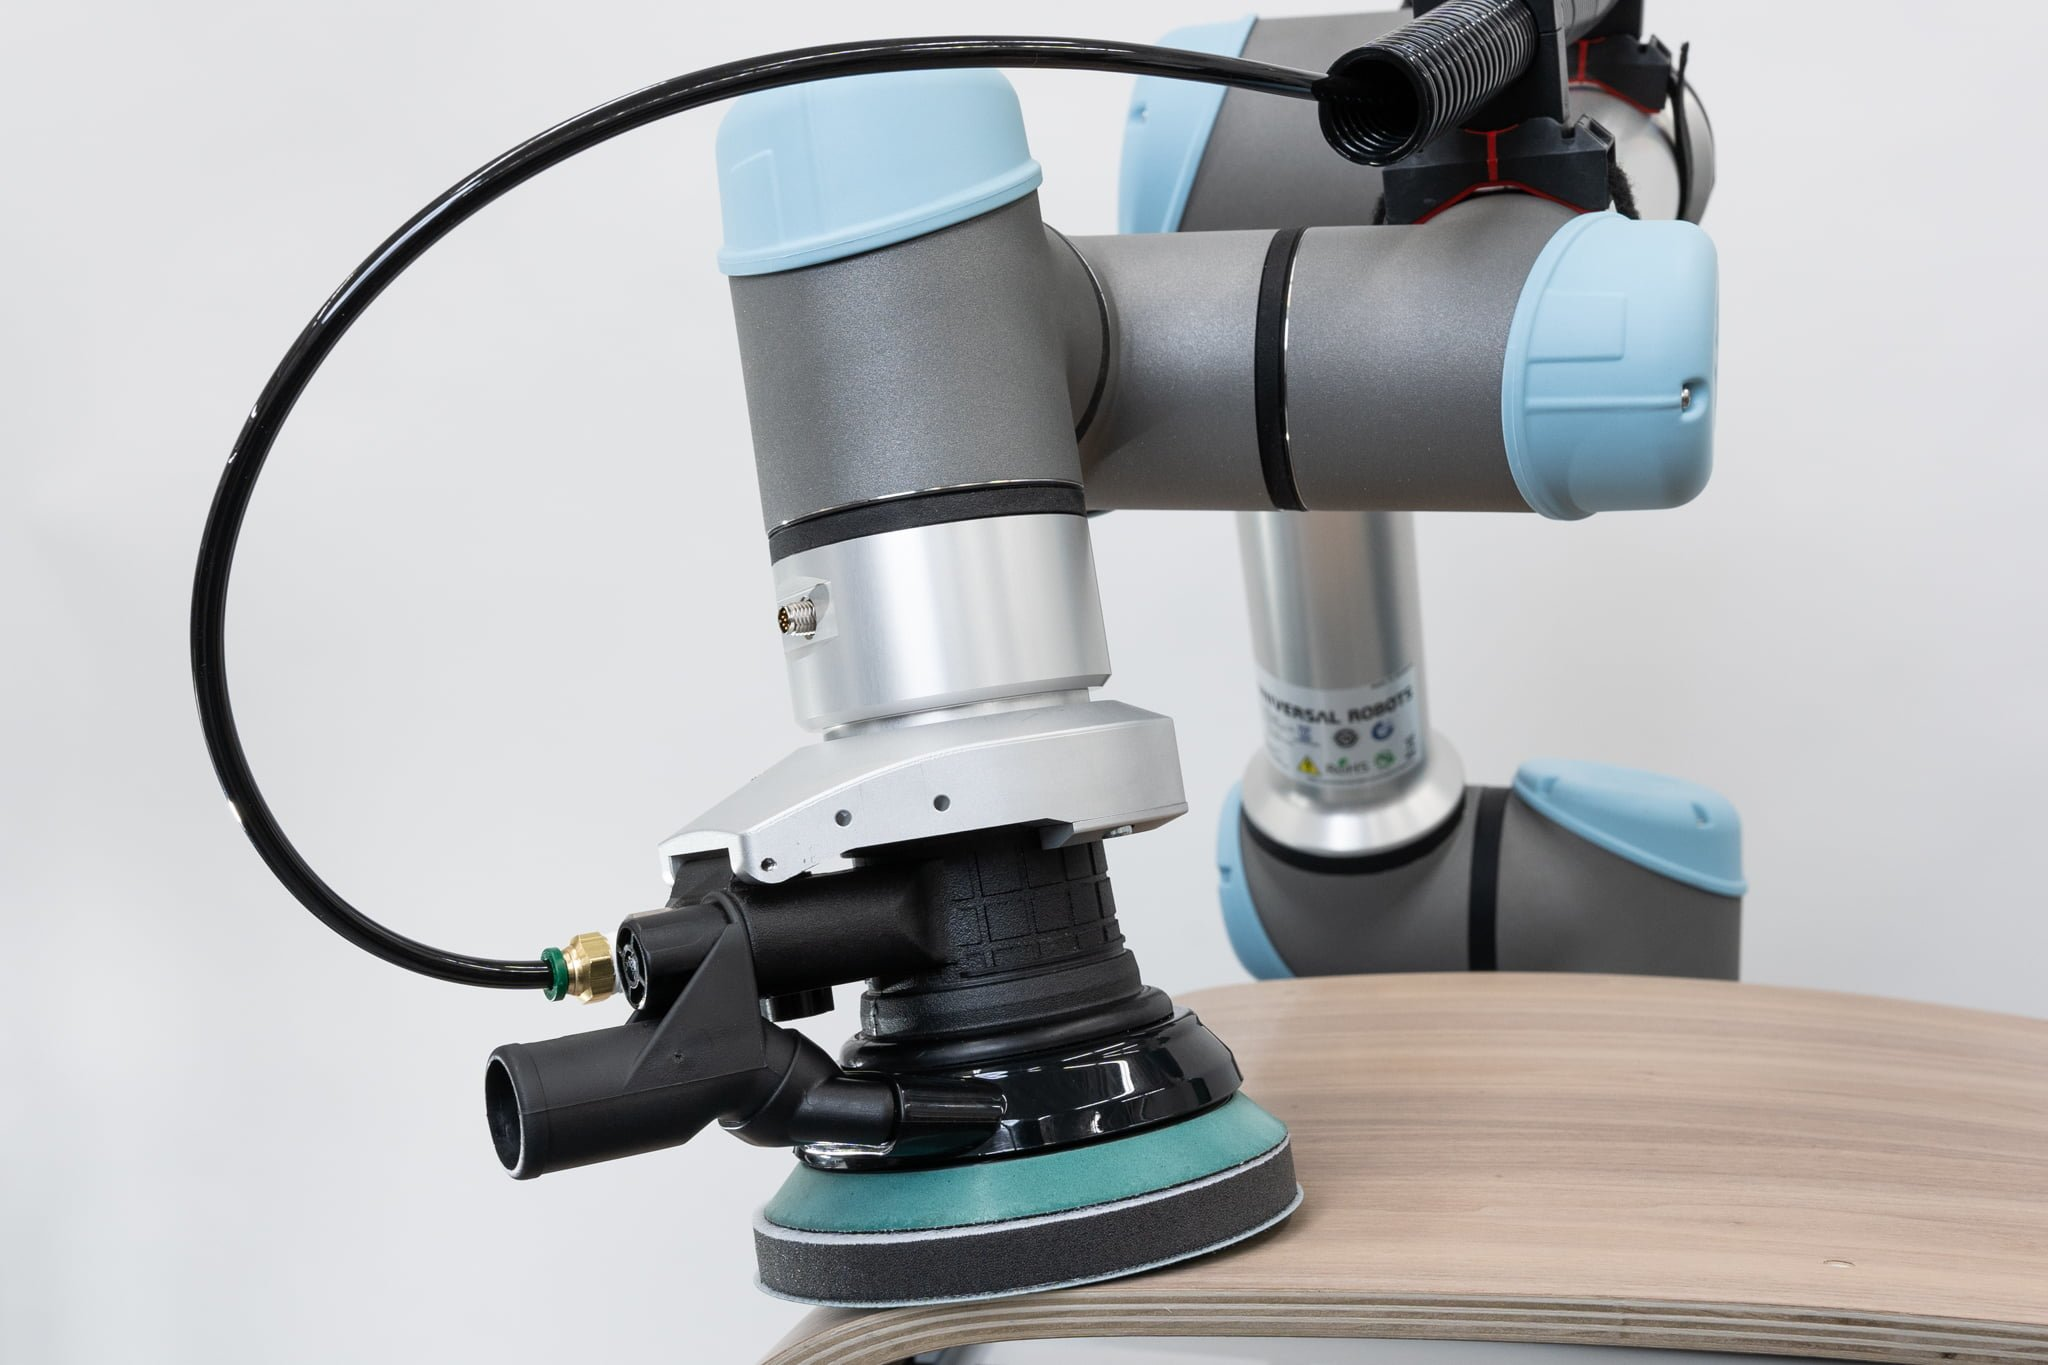
\includegraphics[width=\textwidth]{images/polishing.jpg}
        \caption{Levigatura}
        \label{fig:polishing}
    \end{subfigure}
    ~ %add desired spacing between images, e. g. ~, \quad, \qquad, \hfill etc. 
      %(or a blank line to force the subfigure onto a new line)
    \begin{subfigure}[b]{0.33\textwidth}
        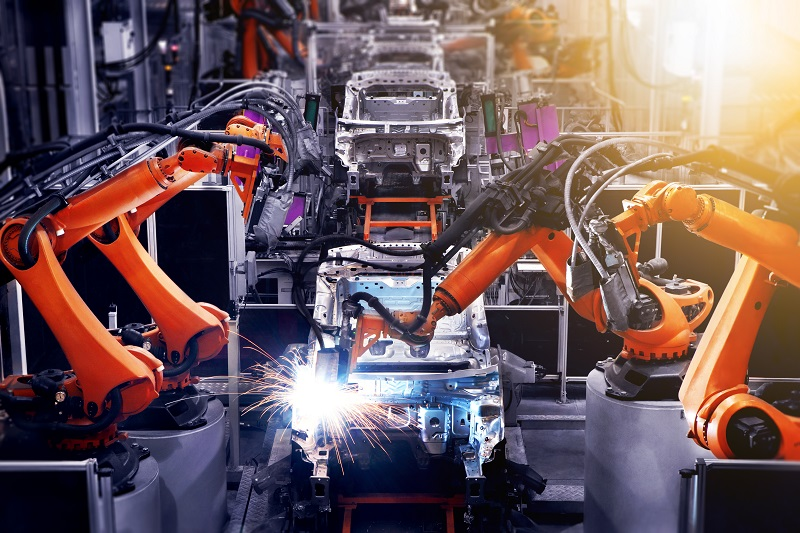
\includegraphics[width=\textwidth]{images/welding.jpeg}
        \caption{Saldatura}
        \label{fig:welding}
    \end{subfigure}
    \begin{subfigure}[b]{0.33\textwidth}
        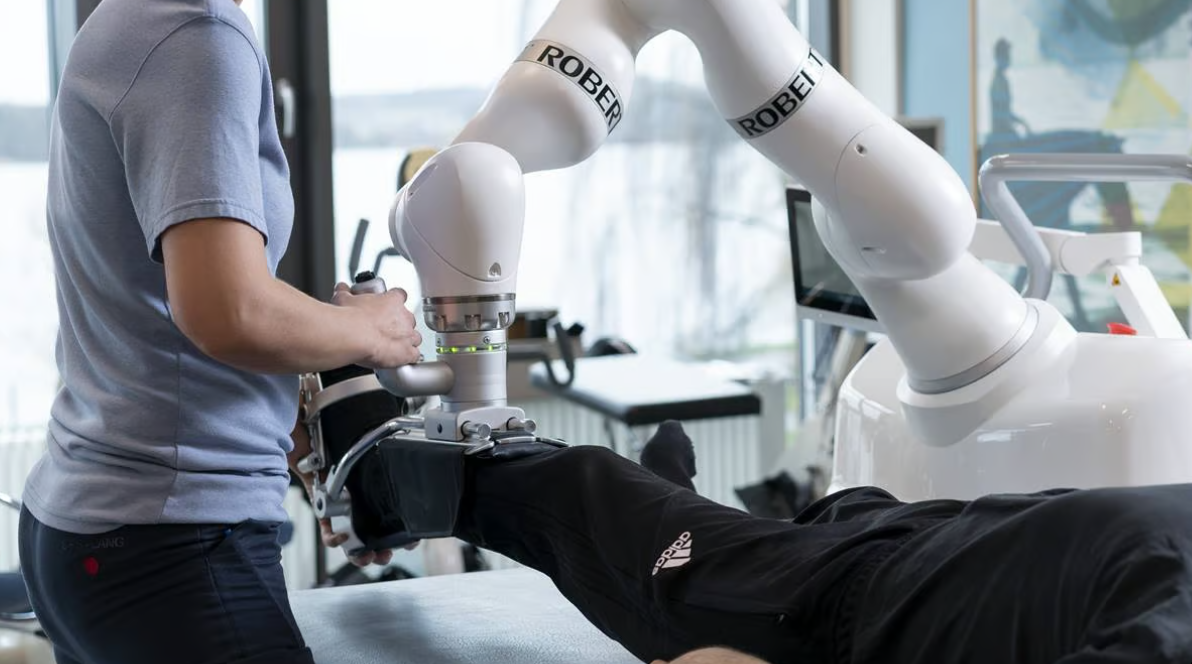
\includegraphics[width=\textwidth]{images/rehabilitation.png}
        \caption{Riabilitazione}
        \label{fig:rehab}
    \end{subfigure}
    \caption{Applicazioni dei sensori coppia-forza}\label{fig:industrial_applications}
\end{figure}
Questi sensori sono in grado di convertire le forze e le coppie applicati ad essi in segnali elettrici che possono essere 
interpretati da altri dispositivi. 
Esistono varie tipologie di sensori coppia-forza, ognuna delle quali ha un diverso meccanismo di funzionamento. 
I sensori \textbf{piezoelettrici}, per esempio, sfruttano la propriet\'{a} di alcuni materiali (cristalli piezoelettrici) 
di generare una carica elettrica se sottoposti a deformazione meccanica. Tale variazione  
pu\'{o} essere misurata per determinare la forza o la coppia applicata.
Il sensore \textbf{FT 300-S} di \textbf{Robotiq} sfrutta proprio questo principio di funzionamento ed \'{e} in grado di misurare 
forze e coppie lungo i sei gradi di libert\'{a} (x, y, z, roll, pitch, yaw). 
Uno dei modelli di robot mainipolatori pi\'{u} utilizzato \'{e} l'\textbf{UR5} di \textbf{Universal Robot}. Si \'{e} scelto di 
utilizzarlo in questo studio, per via della sua flessibilit\'{a} ed efficienza. 
L'UR5, a differenza di altri robot collaborativi, non \'{e} provvisto di sensori coppia-forza integrati. \'{E} stato dunque necessario 
installare l'FT 300-S manualmente. 
In questa tesi verr\'{a} presentata l'implementazione di un sistema di controllo della forza per l'UR5 utilizzando i dati
forniti dall'FT 300-S e il framework di sviluppo \textbf{ROS (Robot Operating System)}.
ROS \'{e} un framework ampiamente utilizzato dalla comunit\'{a} informatica perch\'{e} fornisce strumenti e librerie 
per il controllo e la comunicazione tra le componenti di un sistema robotico. Inizialmente verr\'{a} presentata una panoramica 
sui concetti fondamentali di ROS e sul sensore coppia-forza, mostrando anche due diverse modalit\'{a} di interfacciamento con esso 
(vedi Capitoli \ref{chapter:chapter1} e \ref{chapter:chapter2}).
Nel Capitolo \ref{chapter:chapter3} verr\'{a}, invece, riportata un'analisi per la valutazione delle prestazioni del sensore in termini di 
reattivit\'{a} e precisione. Infine, sar\'{a} presentato il setup sperimentale (vedi Capitolo \ref{chapter:chapter4}) necessario 
allo svolgimento delle applicazioni presentate nel Capitolo \ref{chapter:chapter5} volte a dimostrare l'efficacia
di tali sensori per lo svolgimento di attivit\'{a} industriali, come il \textbf{pick and place} e il \textbf{trasporto collaborativo}.
